%%%%%%%%%%%%%%%%%%%%%%%%%%%%%%%%%%%%%%%%%%%%%%%%%%%%%%%%%%%%%%%%%%%%%%%%%%%%
%% Trim Size : 11in x 8.5in
%% Text Area : 9.6in (include Runningheads) x 7in
%% ws-jai.tex, 26 April 2012
%% Tex file to use with ws-jai.cls written in Latex2E.
%% The content, structure, format and layout of this style file is the
%% property of World Scientific Publishing Co. Pte. Ltd.
%%%%%%%%%%%%%%%%%%%%%%%%%%%%%%%%%%%%%%%%%%%%%%%%%%%%%%%%%%%%%%%%%%%%%%%%%%%%
%%

%\documentclass[draft]{ws-jai}
\documentclass{ws-jai}
\usepackage[flushleft]{threeparttable}
%% \usepackage{subfig}
\begin{document}

\catchline{}{}{}{}{} % Publisher's Area please ignore

\markboth{P.Prasad}{The AARTFAAC Radio Sky Monitor: System Design and Implementation}

\title{The AARTFAAC Radio Sky Monitor: System Design and Implementation}

\author{Peeyush Prasad$^\dagger$, Folkert Huizinga$^\S$, Eric Kooistra$^\ddagger$, Daniel van der Schuur $^\ddagger$, Andre Gunst $^\ddagger$, John Romein $^\ddagger$ and R.A.M.J. Wijers$^\S$}

\address{
$^\dagger$Anton Pannekoek Institute, University of Amsterdam, Amsterdam, The Netherlands, p.prasad@uva.nl\\
$^\ddagger$ASTRON, Oude Hoogeveensedijk, 7991PD, The Netherlands\\
$^\S$Anton Pannekoek Institute, University of Amsterdam, Amsterdam\\
}

\maketitle

\corres{$^\dagger$Corresponding Author}

\begin{history}
\received{(to be inserted by publisher)};
\revised{(to be inserted by publisher)};
\accepted{(to be inserted by publisher)};
\end{history}

\begin{abstract}
The Amsterdam-ASTRON  Radio Transients  Facility And Analysis  Center (AARTFAAC)
array  is  a sensitive,  all-sky  radio  transient  detector  based on  the  Low
Frequency Array (LOFAR).  It generates images  of the low frequency radio sky in
near real-time  with spatial resolution of  10s of arcmin, MHz  bandwidths and a
time cadence of a few seconds. The image timeseries are then monitored for short
and bright radio  transients. On detection of a transient,  low latency triggers
will be  generated for LOFAR,  which can  carry out follow-up  observations.  In
this  paper, we  describe our  heterogenous, hierarchical  design to  manage the
~1.2Tbps raw data  rate, and the ~17TFLOPs of computing  needed.  We discuss the
implementation  of   the  instrumentation,  its  capabilities,   and  show  some
commissioning results.
\end{abstract}

\keywords{Radio Interferometry, Imaging, Radio Transients, Correlators}

\section{\label{sec:Introduction}Introduction}

%\begin{itemize}
% \item What are celestial transients \\
\noindent Transient astronomy  deals with the detection  and characterization of
celestial transients, sources in the  sky whose detectable properties can change
on short timescales.   These explosive events provide insight into  a variety of
astrophysics,  ranging from  emission mechanisms  of jets  to properties  of the
intervening  medium \citep{fender2006lofar,lazio2009dynamic}.  Studies of  short
duration radio  emission from such  objects has  been restricted to  either very
short  timescales  (milliseconds to  seconds,  e.g.   Pulsars[TODO:Ref]), or  to
comparitively  longer timescales  (months to  years[TODO:Ref]) primarily  due to
observational time,  or instrumental constraints,  the former due to  the narrow
fields  of view  of traditional  instruments.  For  time resolved  observations,
radio instrumentation  is generally available  in broadly two classes;  A single
dish  or phased  array beam  formed timeseries  characterized by  high time  and
frequency  resolution,  fields  of  view  of a  few  degrees  but  poor  spatial
resolution,  or interferometric  aperture synthesis  imaging observations.   The
latter  provides  high  spatial  resolution,  but  have  poor  time  resolution,
typically  needing  several hours  of  observation  time  to build  up  adequate
coverage  in the  UV plane  via earth  rotation aperture  synthesis.  The  above
classes roughly translate to coherent  (short timescales) and incoherent (longer
timescales) sources of emission[TODO: Ref].

%\item Current state of the science \\
The serendipitous discovery of a new  class of radio transient termed Fast Radio
Bursts  (FRBs)\citep{spitler2015fast,   thornton2013population}  has  galvanized
interest in the  field.  The detected FRBs are characterized  by high associated
dispersion   measures,  high   brightness  and   short  timescales.    They  are
non-repeating for  the most part. Their  unknown origin requires not  only their
discovery, but also  rapid followup over a large wavelength  regime to establish
emission  phenomena  and  associated  parameters.   A  recent  example  of  this
requirement is the detection by  \cite{stewart2016lofar} of a ~20Jy transient in
60MHz LOFAR  data.  The  last requirement  has led to  the development  of large
field of  view radio sky monitors,  with an aim of  continuously surveying large
parts of the visible sky with shallow sensitivity and at high time resolution. A
trigger  is generated  on the  reliable  detection of  a transient  in close  to
real-time, allowing other telescopes to carry out follow-up observations.

% \item Suitability of low frequency observations \\
% <TODO: Paragraph about  transient sources, some stuff about  spectral indices of
% coherent emission and  expected class of sources, at what  brightness levels can
% we expect to see things (take from Lazio LWA paper).>

% <TODO: Paragraph  summarizing the  current state of  knowledge of  low frequency
% transients: Stewart NCP transient, other  searches at low freq. Conclusion: Need
% for more monitoring.>

% \item What is the AARTFAAC \\
The AARTFAAC  radio transient  monitor is  an All-sky  radio telescope  based on
LOFAR. Its goal is to continuously scan  the skies for bright transients, and on
reliably detecting one, to generate a trigger to other telescopes for sensitive,
broad  band monitoring.   It is  a leading  effort among  a group  of new  radio
telescopes  aiming for  detection  of  bursts of  radio  emission by  continuous
monitoring  of the  low  radio frequency  sky. Other  notable  examples of  such
telescopes are  the Long Wavelength  Array (LWA), \cite{ellingsonLWA1},  and the
Murchison Widefield  Array (MWA), \cite {tingay2013murchison}.   Such telescopes
are characterized by  having moderate resolution and sensitivity  as compared to
contemporary telescopes, but  with extremely wide fields of  view (typically all
sky),  high  availabilities  and  autonomous calibration  and  imaging  in  near
real-time.

The  wide field  of  views necessary  for  an instrument  like  AARTFAAC can  be
achieved by sampling the sky with wide field dipoles. This, however comes at the
cost  of lowered  sensitivity per  receiving element.   An instantaneously  well
sampled UV plane  is needed to generate  a Point Spread Function  (PSF) with low
sidelobes.  Both requirements  can be met by spatially spreading  a large number
of dipoles.  However, this requires  an  order of  magnitude  larger  number  of
elements in the array.  Bringing the resulting large number of data streams to a
central  location,  as well  as  their  correlation  for carrying  out  aperture
synthesis  imaging  in  real-time  thus  poses a  significant  I/O  and  compute
challenge. Further,  the wide fields of  view at the sensitivities  of operation
also result in  direction dependent effects on the incoming  signals, mostly due
to  the ionosphere.  These  pose  a challenge  to  calibration, especially  when
carried out in an autonomous manner.

Apart  from  its  primary  goal  of  trigger  generation  on  the  detection  of
transients, the  AARTFAAC telescope products  find use  in a variety  of science
cases. These  include wide  field ionospheric monitoring  via apparent  flux and
position  variations of  calibrator  sources, Solar  monitoring, RFI  surveying,
LOFAR beam model validation etc.

The incoming  sampled voltages  pass through  various signal  processing blocks,
resulting  in the  generation of  light curves  for sources  in a  timeseries of
images.  The estimation of spatial coherences requires the reordering of data to
make optimum usage of compute resources.  Thus, the functioning of the telescope
depends  on the  optimization of  the  data transport,  data reorganization  and
computing using available resources.  An  advantage of having an operating model
consisting  of signal  processing blocks  operating on  signals sampled  at high
resolutions is  the configurability  of the  telescope into  different observing
modes, as well as the tapping off of data from an upstream location.  The latter
ability makes a piggy-back instrument  like the AARTFAAC possible.  An important
resource to optimize is the development time for each data routing or processing
block, and this has been taken into consideration in the AARTFAAC.

%\item Paper description \\
In  this paper,  we describe  the  AARTFAAC telescope  system architecture,  its
instrumentation,  and  the commissioning  of  its  various subsystems.   Section
\ref{sec:aartfaac_array} describes the array and the receiving antenna elements,
its  relationship  with LOFAR,  and  introduces  the  full architecture  of  the
instrument.    Section   \ref{sec:station_hardware}   describes   the   hardware
implementation in  the field which  allows creating a  data path in  parallel to
LOFAR. This  makes AARTFAAC processing independent  of LOFAR to a  large extent.
In Section \ref{sec:gpucorr}, we describe the implementation of a real-time, GPU
based  correlator  for  AARTFAAC,  while  Section  \ref{sec:calim}  details  the
real-time,   autonomous  calibration   and   imaging  implementation.    Section
\ref{sec:acontrol} describes our  control system for the  full instrument, which
also interfaces with LOFAR.  In Section \ref{sec:results} we present performance
metrics of the instrument as a whole.
%\end{itemize}

\section {\label{sec:aartfaac_array}The AARTFAAC array}
We  begin by  summarizing the  subsystems of  the LOFAR  telescope relevant  for
AARTFAAC processing in  Section \ref{subsec:lofar}, and then  elaborating on the
scheme for creating a coupled data path for independent processing by AARTFAAC.

\subsection {\label{subsec:lofar} LOFAR telescope architecture}
The   LOFAR   telescope  \citep{van2013lofar}   is   a   new  generation   radio
interferometer  covering  the frequency  range  from  10-90 MHz  using  inverted
V-dipoles known  as Low Band  Antenna (LBA), and  from 110-240 MHz  using Bowtie
dipoles,  also known  as  High Band  Antenna (HBA).   The  antenna are  linearly
polarized, being made  up of orthogonally placed dipoles.  The  LBA dipole has a
sensitivity pattern with  a 6dB field of  view of about $120^o$  at 60MHz, while
the HBA dipoles first undergo an analog phasing within a 4x4 tile, which results
in  a field  of view  of  about $20^o$  at 150  MHz  [TODO: Ref].   Due to  this
restriction,  the  AARTFAAC  array  utilizes  only  the  LBA  component  of  the
telescope.

The  telescope itself  consists of  a  large collection  of antennas,  spatially
organized  into several  'stations', each  of 48  dual-pol antennas  spread over
~60m.  The  stations are  laid out  in a dense  core: 24  stations within  a 2km
radius, with the long  baselines made up using stations upto  a 1000km away from
the core. 

In the  regular LOFAR station  level processing,  the sampled bandwidth  of each
dipole  is split  into subbands,  which are  then digitally  phased in  hardware
towards the  direction of  an astronomical  source to form  a station  beam. The
phasing is  updated periodically to track  a position in the  sky. The resulting
beam is  then transmitted over optical  fiber to a central  location for further
interferometric processing with other stations.

\subsection {\label{subsec:aartfaac}  The AARTFAAC system}
\begin{figure*}[htbp]
\centering
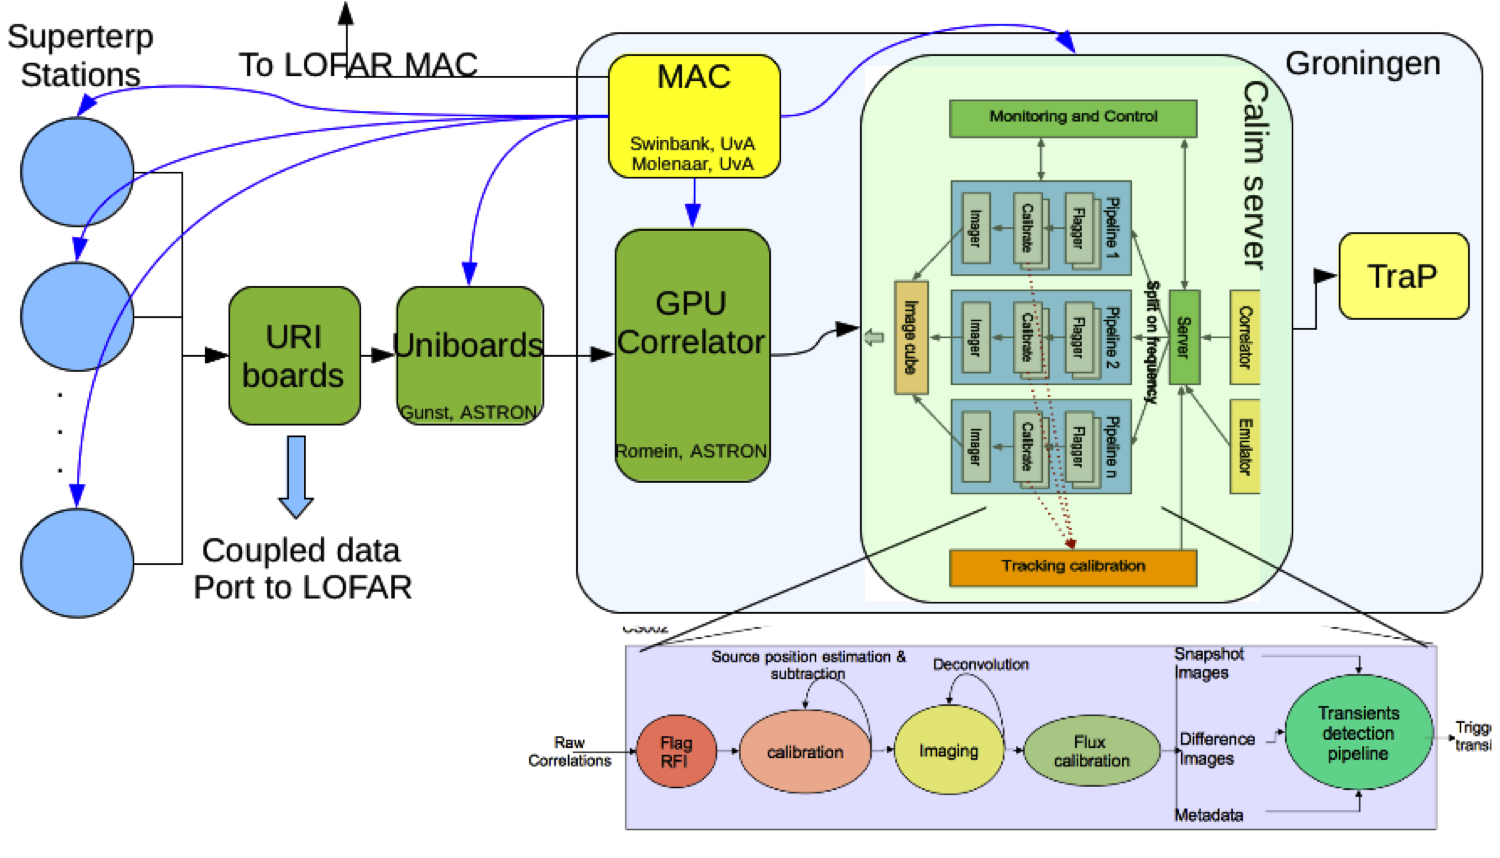
\includegraphics[width=1\textwidth]{Figs/overall_afaac_Arch_blks.png}
\caption {Overall  architecture of the  AARTFAAC all-sky monitor  depicting each
  processing subblock, along with the Monitoring and Control (MAC) system. }
\label{fig:afaac_arch}
\end{figure*}

The AARTFAAC  array consists of  12-stations from within  the core of  the LOFAR
telescope, with interdipole distances ranging  from (TODO) within a station, and
a maximum of TODO across stations.  Due  to the requirement of dipole level data
in order to achieve all-sky imaging, the AARTFAAC creates a coupled data path to
an independent processing  architecture, prior to the phasing up  of the dipoles
within  a  station in  the  LOFAR  processing  flow.  This  allows  simultaneous
observing with  LOFAR, leading to  high availability  of the AARTFAAC  system. A
subset  of the  available  subbands  are correlated  in  a  dedicated GPU  based
correlator in  real-time.  The  estimated visibilities are  sent over  TCP/IP to
dedicated servers for carrying out  the autonomous and real-time calibration and
imaging.  The generated  images are further sent to a  software pipeline for the
actual detection of transients, based on  comparison of the image timeseries.  A
(planned) trigger  generation subsystem  will publish  reliable triggers  in the
form  of VOEvents  \cite{williams2006voevent},  which can  be  claimed by  other
telescopes    to    observe    candidates     with    high    sensitivity    and
resolution.  Fig.   \ref{fig:afaac_arch}  shows  the  overall   AARTFAAC  system
architecture, including the  data routing and processing blocks, as  well as the
control and monitoring flow.

The station consititutes  the first component of the radio  sky monitor, and are
the only components shared with LOFAR.  The AARTFAAC monitor consists of further
subsystems which are independent of  LOFAR processing.  Its overall architecture
is shown schematically in Figure  \ref{fig:afaac_arch}, and illustrates the main
processing subblocks of the instrument.   To summarize, a user selectable subset
of subbands  from every dipole  is transferred as  UDP packets over  a dedicated
10Gbit fiber connection  to the central processing systems.   These are received
by  a streaming  software correlator  implementation which  aligns the  data and
estimates  the spatial  covariance matrix  between every  pair of  dipoles.  The
generated visibilities  are streamed  over TCP/IP to  a calibration  and imaging
pipeline component  which carries out  autonomous imaging.  The images  are then
analyzed    by   a    software    tool   (The    Transients   Pipeline,    TraP,
\citep{swinbank2015lofar}), which  extracts the  light curves of  sources within
the image, and analyses them for variability using a number of parameters.


\begin{figure*}[htbp]
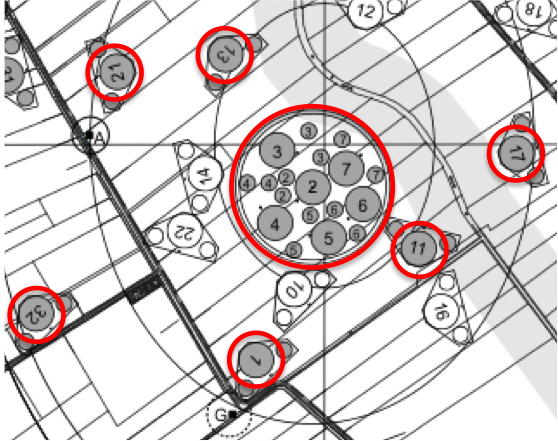
\includegraphics[width=0.5\textwidth]{Figs/afaac12_arrayconfig.png}
\caption{The spatial distribution of AARTFAAC-12 stations within the core of LOFAR stations.}
\label{fig:afaac12_arrayconfig}
\end{figure*}

\begin{wstable}[h]
\caption{Specifications of the AARTFAAC All-sky radio monitor.}
\begin{tabular}{@{}cccc@{}} \toprule
Parameter & Specification & Units & Comment\\ \colrule
Frequency range & 10-90 & MHz & Assuming LBA processing  \\
Processed bandwidth & 6.25 & MHz & Processing 32 subbands \\
Maximum baseline & 1500 & m & In LBA\_OUTER station array configuration\\
Resolution & 0 & arcmin & \\
Usable field of view & 130 & deg & SNR of TODO \\
Sensitivity & TODO & Jy & 8 Subbands gridded on a common grid \\

\end{tabular}
%% \begin{tablenotes}
%% \item[a] Sample table notes.
%% \item[b] Sample table notes.
%% \end{tablenotes}
\label{tab:afaac_specs}
\end{wstable}

\noindent  \textbf {Array  configuration:} The  choice  of the  subset of  LOFAR
stations used  in the AARTFAAC system  is dictated primarily by  imaging quality
and sensitivity, as well as due to constraints on the latency of calibration and
imaging. The central six stations of  the LOFAR telescope (called the superterp)
form a  densely sampled UV plane,  and are ideal  for wide field imaging  due to
their  being co-planar  to  high  accuracy (centimeter  level).   The outer  six
stations provide  higher sensitivity and resolution,  and have been chosen  as a
compromise  between  the  UV  coverage  and the  extra  processing  due  to  the
W-component.  The salient  features of the LBA\_OUTER  station configuration for
the  chosen stations  are shown  in table  Table \ref{tab:afaac_specs}.   Figure
\ref{fig:afaac12_arrayconfig}  shows the  LOFAR stations  that are  part of  the
AARTFAAC system.

We describe the various subsystems making up the AARTFAAC All-sky monitor in the
following sections.

\section {\label{sec:station_hardware} Remote Station Level Processing:} 
Remote Station processing  refers to instrumentation installed in  the field and
coupled to the receiving antennas post balun. The Receiver Unit (RCU) boards and
the Remote Station Processing (RSP) boards  carry out signal processing for both
LOFAR and  AARTFAAC.  The  Uniboard-RSP Interface (URI)  board and  the Uniboard
(UNB) \ref{}  based data router  are specific to  the AARTFAAC signal  flow, and
carry out data shuffling and transport operations.\\

\noindent  \textbf {Signal  processing:} The  RCU board  carries out  the analog
signal conditioning of the voltage received from a dipole, followed by base band
digitization at  200MHz with a 12-bit  resolution. The RSP \ref{}  board carries
out the FPGA based first stage, 1024-tap polyphase filter bank implementation on
each  dipole input,  and this  processing is  common to  the LOFAR  and AARTFAAC
telescopes. It  analyzes the sampled  voltage timeseries into a  complex voltage
spectrum  of 512  subbands. Thus,  the  entire analog  band of  the LBA  between
10-90MHz is available for further processing. The output, for a set of 1024 real
voltage samples, consists of a complex  number per subband, with a 2s complement
16-bit representation of  the real and imaginary components. A  single RSP board
can handle the processing of sampled  data from 4 dual polarized dipoles.  Since
a LOFAR station is made up of  48 dual polarized dipole antennas, 12 RSP boards
are required per station.  This is shown in Fig. \ref{fig:afaac_station_hw}. For
LOFAR, these subbands are further processed  in the RSP boards to form spatially
directed station beams.\\

%% Station level  beamforming in  a particular  direction requires  calculating the
%% weighted sum of  all dipoles of the same polarization,  with the applied weights
%% being dependent on  the direction of beamforming.  Each  RSP board fundamentally
%% generates the  beamformed product for  its 4  client dipoles for  every subband.
%% These are termed  as 'beamlets'.  The necessary exchange of  beamlets with other
%% RSP boards to  create the station beam is achieved  via the interconnect between
%% the various RSP boards.\\

%% Each data  product from the RSP  signal processing is encapsulated  in a packet,
%% and marked with a datatype magic number. This allows differentiation between the
%% generated data products.

\noindent \textbf {Interconnect:} A ring network consisting of four 2 Gbps links
interconnects the 12 RSP boards of a station to each other by daisy chaining the
serial I/O  links to the  RSP boards to  each other. It  is used to  carry LOFAR
specific data products, along with the raw AARTFAAC subbands. Of the total 8Gbps
bandwidth  of the  ring  network,  about 6 Gbps  is  occupied  by LOFAR  specific
products,  with  the  remaining  bandwidth carrying  per  dipole  subbands  used
exclusively for AARTFAAC processing.\\

\noindent \textbf  {Available bit modes:} The  bit mode refers to  the number of
bits  utilized in  the  quantization of  the components  of  the complex  number
representing a subband signal.  Thus, the system offers the ability to trade off
dynamic range in  the polyphase filter bank outputs with  the number of subbands
available  for further  processing.   This is  done by  reducing  the number  of
allocated bits  to the  real and  imaginary components  of the  subband outputs,
leading  to an  increased  number of  subbands.  The  reduction  is carried  out
statically, based on a previous analysis  of the observing environment.  The bit
mode of  AARTFAAC can be set  completely independently of LOFAR's  choice of bit
mode. The choice between the various bit modes depends on the RFI environment of
the observation.  An 8-bit complex representation of the filterbank subbands are
found to  be adequate for almost  all observing conditions except  during severe
RFI.\\


\noindent \textbf  {Sampling clock and  Timing:} This sub-system is  shared with
LOFAR. A  clock distributer board (SyncOptics)  \ref{} at the center  is used to
distribute  a 10MHz  reference  to every  one  of the  24  core LOFAR  stations,
including the 12  AARTFAAC stations.  The 10MHz reference is  generated by a GPS
discplined  Rubidium  frequency   standard,  and  is  fed  into   a  Timing  and
Distribution  Board at  the station.  This board  generates the  200MHz sampling
clock required by the RCUs, and is also  used for the data processing at the RSP
boards. It  ensures that  an identical  (hence coherent) clock  is used  for the
sampling of data from the AARTFAAC stations.\\

The absolute time is communicated to the  RSP boards on station reset by the LCU
(local control  unit) as a 64-bit  timestamp counter. The RSP  board then starts
using this 64-bit timestamp at the start  of the next second, indicated by a PPS
(pulse per second)  signal from the GPS timing.  Once  set, the station hardware
updates  this counter  on a  derivate of  the available  200MHz reference,  thus
ensuring that the  absolute time is embedded  in the data with a  precision of a
single subband's timesample ($\sim5\mu sec$). All  further aligning and timing of
the incoming data is carried out based on this embedded timestamp.\\

\noindent  \textbf  {The  Uniboard-RSP  Interface (URI)  board:}  This  AARTFAAC
specific board creates  a coupled path for the subband  data by segregating them
from the LOFAR specific data products  flowing on the station ring network. This
is implemented by interfacing  the serial I/O links of 4 RSP  boards to a single
URI  board, which  interrogates the  incoming packets,  and selects  the subband
outputs based on packet type. Thus,  the URI board ensures high availability via
simultaneous operation of LOFAR and  AARTFAAC.

This block further implements the first stage of the overall transpose operation
required  to  bring  coincident  data  of  all  dipoles  to  consecutive  memory
locations.  It  does so by statically  routing upto 9 subbands  from all dipoles
available on the 4 RSP boards to a single output lane. Thus, while each incoming
link contains 36 subbands from 8 dipoles, each outgoing link contains 9 subbands
from    32    subbands.     This    operation    can    be    seen    in    Fig.
\ref{fig:afaac_station_hw} in the  dataflow layout between the URI  and the UNB,
which shows the collation  of data from 9 subbands for 32  dipoles onto a single
data  link.   All together,  three  URI  boards  are  adequate to  transfer  and
transpose 36 subbands at 16-bits into the Uniboard based router.\\

\noindent \textbf  {The Uniboard based data  router:} This data routing  unit is
the  interface between  the station  level instrumentation  and the  next signal
processing unit, the correlator. The board  consists of 4 upstream FPGAs (called
backnodes)  connected  to   the  URI  boards,  and   4  downstream  FPGAs(called
frontnodes) to  connect to the correlator  over long haul fiber  links.  Each of
the backnode FPGAs receives 9 consecutive subbands out of the 36 subbands in the
URI board output.  However, output bandwidth constraints limit  the backnodes to
transferring 8 of the 9 subbands onwards.

A second level  of data rerouting is  carried out at this stage  such that links
from the 3 different URI boards (each containing 9 subbands from 32 dipoles) are
connected to  the same backnode.  This allows the  backnode to collect  the same
subbands from all 96  dipoles making up the station, into  a single output link.

These data are transported to a  single Frontnode FPGA.  The latter encapsulates
the  data into  a UDP  packet  which is  transmitted  on a  long haul  10Gigabit
Ethernet interface  to the  remote correlator.  A  single Uniboard  operates two
10Gbps links  to the central processing  machines, located at the  University of
Groningen about 50Km away.  Each link  carries about 9.8Gbps of data, consisting
of 16 subbands of 16bits from all dipoles in the station.\\

\noindent  \textbf {Data  rates  and bandwidth  limitations:  } The  fundamental
limitation  to  AARTFAAC  processed  bandwidth is  presented  by  the  bandwidth
available  on  the ring  network,  and  depends  on  the bit-mode  chosen.   The
bandwidth available  to AARTFAAC is  limited to 36  subbands in 16-bit  mode, 72
subbands in  8-bit mode, 108 subbands  in 5 bit  mode, or 144 subbands  in 4-bit
mode.  A  random selection of  subbands from the  available 512 can  be inserted
into the  available AARTFAAC slots on  the ring network.  This  selection can be
made via  manipulation of the control  registers of the RSP  board.  This allows
AARTFAAC to achieve high sensitivity by placing subbands contiguously, and later
integrating them, while at the same  time achieving spectral coverage by placing
subbands to sample a larger extent of the analog spectrum.\\

%% The stations operate on a fixed sampling  clock of 200 MHz, leading to an output
%% rate of ~12  Mbps per dual polarised dipole antenna  per 16-bit complex subband.
%% The limited ring network bandwidth of a  station allows only 36 of the available
%% 512 subbands of 16-bits from all dipole antennas (total bandwidth ~20Gbps) to be
%% carried to  the URI board.  The  station Uniboard further restricts  the sampled
%% bandwidth to match its output bandwidth into 2x10Gbps links.  Of the incoming 36
%% subbands, only  16 are forwarded  for correlation.   Each 10Gbps link  carries 8
%% subbands, corresponding to ~4.5Gbps of data.

\noindent \textbf {Monitoring and Control  interface:} Every station is equipped
with a  Local Control Unit  (LCU), which is an  embedded system running  a Linux
operating system.  These systems are networked  to the LOFAR control system, and
also act as Network Time Protocol  (NTP) clients. Thus, their absolute times are
aligned to  better than a  few milliseconds. The  control of the  remote station
electronics  consists of  two layers.   Command and  status registers  have been
opened up at the FPGA level.  These can be accessed via a dedicated and separate
control Gigabit Ethernet  interface. Each station is also equipped  with a Local
Control  Unit  (LCU)  computer  which  provides  an  abstraction  layer  to  the
hardware. All control  and monitoring commands from a global  control system are
addressed  to the  LCU,  which provides  a  tool that  can  access the  hardware
registers  via a  driver, which  ultimately communicates  the commands  over the
Gigabit ethernet control link to the RSP boards of the station.

% \begin{figure*}[htbp]
% \centering
% 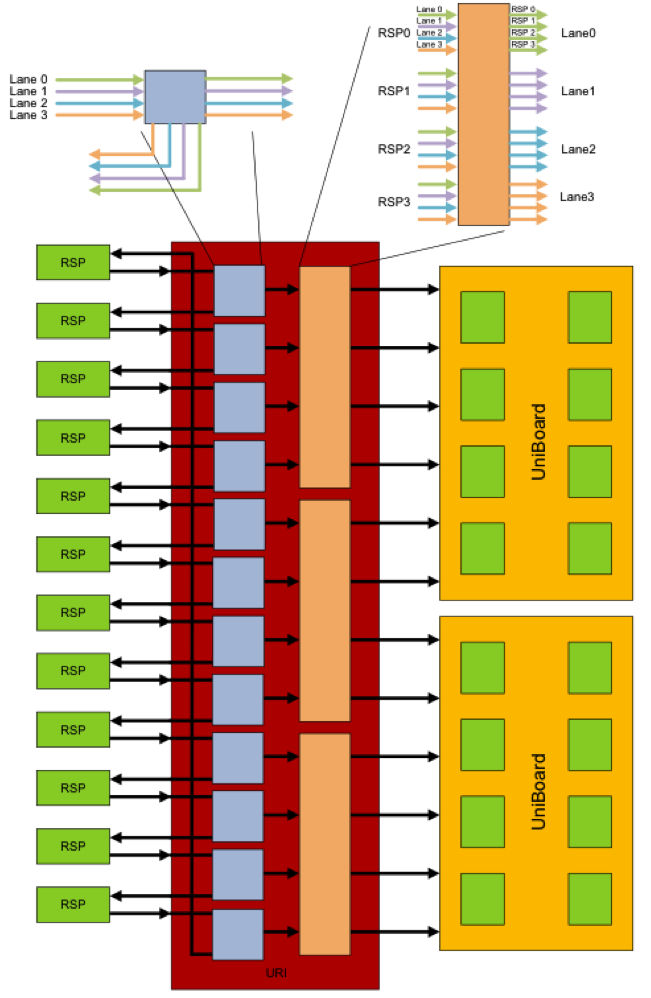
\includegraphics[width=0.75\textwidth]{Figs/station_hw_proc_afaac.png}
% \caption{The station level hardware changes  allowing creation of a coupled data
%   path for AARTFAAC data flow.}
% \label{fig:afaac_station_hw}
% \end{figure*}

% Figure \ref{fig:afaac_station_hw} depicts the  station level ring network, whose
% bandwidth is shared between the beamformed  subbands as well as the dipole level
% subbands. The ring network bandwidth constrains the processed AARTFAAC bandwidth
% to  a fundamental  maximum of  36 16-bit  subbands, or  about 7  MHz, while  the
% Uniboard  interface further  restricts the  bandwidth to  8 subbands  per 10Gpbs
% output link. The URI boards in combination  with the uniboards carry out a first
% level of the incoming data transposition.

\section {\label{sec:gpucorr} The AARTFAAC real-time correlator}
\begin{figure*}[htbp]
\centering
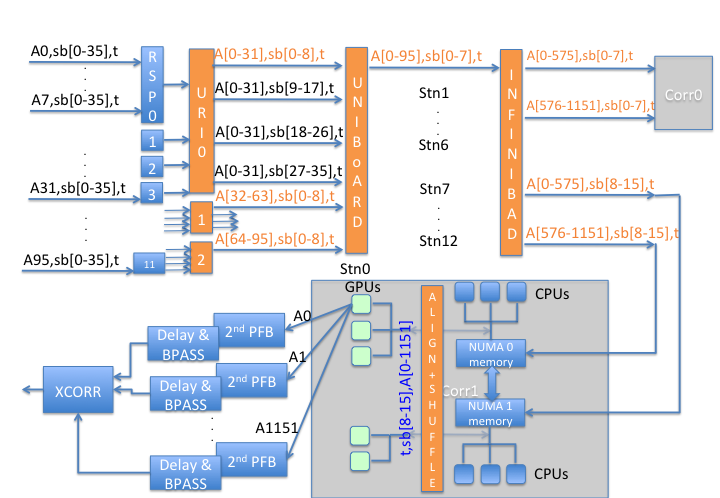
\includegraphics[width=1\textwidth]{Figs/data_routing_transform_hierarchy/Slide1.png}
% \caption{The GPU  correlator implementation  using a pair  of Xeon  class server
%  machines hosting AMD GPUs}
\caption{The hierarchical  data processing and routing  necessary for optimizing
  correlator  compute  performance   on  GPGPUs.  Here,  the   flowing  data  is
  represented by the triad of $[Ai,sb[i-j],t]$, where Ai refer to an individual
  dipole, sb[i-j] refer  to the range of  processed subbands, and t  refers to a
  time  sample.  The orange  blocks  correspond  to hierarchical  elements  that
  shuffle data }
\label{fig:afaac_station_hw}
\end{figure*}

% \begin {itemize}
% \item  What does  the correlator  do\\  
The correlator  subsystem estimates the  spatial coherence between all  pairs of
dipoles in the system, per frequency  channel. With 12 stations, each containing
48 dual-polarised  antennas, the  total number  of dipoles  is 1152,  making the
correlator one with the highest number of spatially distinct input streams among
contemporary instruments.  This is  the most computationally intensive subsystem
of  the  pipeline.   Its  input  is formed  of  the  subbanded  complex  voltage
timeseries from  each polarization of every  antenna.  The output consists  of a
timeseries of dipole array covariance matrices  with a chosen time and frequency
averaging.

% \item The correlator  requirements for AARTFAAC \\
The correlator ingests about 9.6 Gbps per station in real-time, corresponding to
16  subbands of  16bits for  each  of the  1152  dipoles.  It  needs to  produce
channelized data  from the subband  inputs due  to requirements of  flagging and
calibration. The resulting  computation is theoretically about  ~17TFLOPs, to be
carried out  in real-time,  with minimum  latency.  A  major requirement  was to
minimize  development  effort,  which   effectively  eliminated  an  FPGA  based
approach.

% \item Motivating the GPGPU approach\\
Of the available approaches, an heterogenous GPGPU approach turned out to be the
best   match   between   our   requirements   of   ease   of   development   and
performance.  Compared to  multi-core CPUs,  DSP architectures,  GPUs have  been
found to have the best performance and energy efficiency for algorithms relevant
to radio astronomy \cite{romein2016comparison}.  The correlation operation has a
low Arithmetic  Intensity, implying  that the  data brought to  a device  ALU is
operated on only a few times.  This, combined with the relatively restricted I/O
bandwidth between the host CPU and the  device GPU, has been used as an argument
against using GPGPU systems for  correlation. However, with increasing number of
signal  sources,  the  I/O  requirements   scale  linearly,  while  the  compute
requirements scale quadratically. Thus, a large enough input system can make the
application compute bound. This is the  case withthe AARTFAAC system. The latest
GPUs come close to meeting our requirements.\\ The LOFAR correlator architecture
needs real-time  processing to reduce the  large volume of data  being produced.
Its implementation  is based  on a  hybrid architecture  using GPGPUs  and CPUs.
However, it  deals with  far fewer  station input streams  due to  station level
beamforming.


% \item Functional blocks \\
The signal processing blocks necessary to achieve the correlator specs are shown
in Fig. TODO.  After the incoming subbanded data from each station is aligned, a
Polyphase filter bank is implemented  in order to increase frequency resolution.
The resulting channels are then delay  compensated for the fixed cable delays in
the system, as  well as for the  bandpass response of the  first stage Polyphase
filter  bank.  Following  this, signals  from corresponding  timeslices for  all
stations are correlated. The generated covariance matrix is then written out for
further processing.
% \end {itemize}

\subsection  {Implementation  Hardware  architecture:} 
The AARTFAAC  correlator has  been implemented  using a  GPGPU approach,  with a
server class  machine utilizing a  GPU device  for carrying out  the computation
necessary  for  the correlation.   The  host  CPU  based  machines acts  as  the
interface between  the stations and  the GPU  devices.  They implement  the data
reception, and arbitrate the data distribution between different GPUs. They also
carry out the last stage of the  transform operation to optimize the data layout
for computing the spectral coherence on a GPU.

The  implementation  consists  of  two identical  machine  configurations,  each
capable  of processing  16  incoming  subbands from  12  stations. Each  machine
consists  of  dual Xeon-class  processors  with  24  cores  each. The  CPUs  are
connected to 32 GB  of memory each, operating in a  NUMA configuration. Five AMD
FirePro S10000 GPU cards are available  per machine, interfaced to the CPUs over
8x16bit PCIe lanes (TODO: Verify correctness). To receive the ~5Gbps data output
from each  of the 12 stations,  the server is equipped  with 2x40Gbps infiniband
interfaces, each  receiving data from 6  stations, and also carrying  the output
products to downstream processors.

\noindent \textbf {High bandwidth switch:}  An infiniband high bandwidth switch,
in combination with the Uniboard data router,  is utilized to carry out the last
stage transform of the  per dipole data stream. This results  in the same subset
of subbands from all 12 stations being transmitted to the same server, 6 to each
of the infiniband  interfaces.  The Backnode FPGAs of  the Uniboards encapsulate
data  such that  a  subset of  8  subbands  from 6  stations  have an  identical
destination IP address of one of the interfaces.

\noindent \textbf  {NUMA domains:}  A  Non Uniform  Memory Access  (NUMA)  CPU and  memory
architecture is necessary in order to manage the high I/O over infiniband and to
the GPUs,  as well as to  manage the last  stage data exchange of  the 6-station
data  between CPUs  controlling the  two infiniband  cards (see  Fig. TODO).   A
single  machines resources  are organized  into two  NUMA domains.   Each domain
includes  an  infiniband  interface,  a  set of  processing  cores,  the  memory
associated with  them. However,  the split  of the  5 GPU  cards cannot  be made
symmetrically between the two domains, leaving one domain with 3 GPUs, while the
other domain as 2 GPUs.  The NUMA  domains allow binding of threads handling I/O
and  processing to  preferred CPU  cores.  This  also prevents  thread migration
which  furthers data  locality,  and  allows routing  of  network interrupts  to
preferred cores. This is essential for ensuring bounded latency.

Fig. \ref{fig:afaac_station_hw}  shows the data routing  and computing hierarchy
in the AARTFAAC system.

\subsection {Implementation of functional  blocks:} 

In this  section, we provide a  description of the implementation  of individual
functional blocks on our target hardware.\\
\noindent \textbf {CPU Data alignment and transpose:} The raw data input packets
from individual stations need to be collated for an entire integration period in
host memory,  before being  shipped to the  GPUs for correlation.   4 of  the 24
available processor cores in a NUMA domain  are allocated for the execution of a
thread pool for the infiniband I/O  handling. Six Bounded threads are created to
run on  the 4  cores, one per  input station.  The  incoming subbands  from each
station  need to  be  time aligned  before further  processing.   They are  also
organized in the {Station, Time, Subband}  order by the upstream hardware, while
it is more efficient to reorder them into {time, Subband, Station} order for the
correlation process.\\  Both effects  are achieved  by setting  up a  large, per
subband 3-D buffer for the incoming  data, with the input threads converting the
incoming data  from signed integer to  float, and placing them  into the correct
time,  station and  subband  slot within  the global  buffer.   This last  stage
transpose    is   shown    schematically   associated    with   the    CPUs   in
Fig. \ref{fig:afaac_station_hw}.   Note that  half the stations  are received
via the inifniband interface on the second  NUMA domain, and an exchange of half
the subbands  takes place between  the two NUMA  domains. The number  of missing
slots  is also  logged, and  is  used to  generate  a weighting  matrix for  the
estimated integrated  visibilities. The aligned and  transposed visibilities are
then ready to be transferred to a GPU's global memory for further processing.

The interface to the openCL runtime is  via a Queue onto which available GPUs in
the same NUMA domain  line up for claiming a subband's  data.  Once claimed, the
raw data  is transferred  asynchronously to  the GPU  device memory  for further
processing.   A  GPU  thread  is  created  to  handle  the  processing  of  data
corresponding to the  integration block of each subband  separately.  The OpenCL
runtime compiles the GPU kernel code  in runtime, and produces the assembly code
to be executed by  the GPU's Compute Units. Neither the  Texture memory, nor the
render outputs  of the GPU architecture  are used. To optimize  performance, the
work-unit splits the data such that only the register file per CU is utilized at
every stage.\\

\noindent  \textbf {Polyphase  Filterbank kernel:}  The first  signal processing
block  is  a  PolyPhase  filterbank,   applied  onto  the  single  subband,  and
constituted  of a  256-tap FIR  filter, followed  by a  1-D complex  FFT of  the
subband timeseries.  The FFT is carried  out using an openCL  library, while the
FIR  filter  is implemented  to  maximize  the usage  of  the  GPU compute  unit
registers. The output is saved in the device global memory.\\

\noindent \textbf  {Delay and Bandpass  compensation kernel:} Subsequent  to the
PolyPhase filter bank implementation, a delay compensation is applied to account
for the fixed cable  delays of the dipoles with respect  to a reference antenna.
These delays are obtained via a separate calibration, which is typically carried
out at  a cadence  of a  few months.   The delays  are available  in calibration
tables,  and the  frequency resolution  is high  enough to  apply them  as phase
rotations   of  the   visibilities.   The  first   stage  polyphase   filterbank
implementation in the RSP board  results in a deterministic amplitude modulation
on the subband bandpass, and leading  to unequal powers in each subband channel.
This  is demodulated  via the  application of  a fixed  amplitude correction  by
applying channel  dependent weights. The resulting  data is brought to  the user
desired frequency resolution by integrating the channels.\\

\begin{figure*}[htbp]
\centering
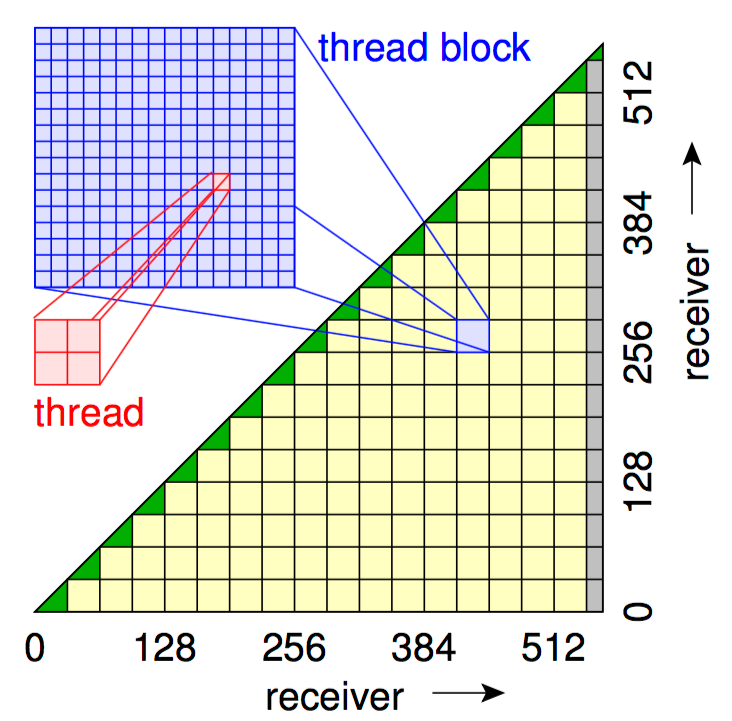
\includegraphics[width=0.5\textwidth]{Figs/ACM_spatial_split.png}
\caption {Depiction of the splitting of each output cell of a covariance matrix into triangles, rectangles and squares, which are computed by a compute unit of a GPU. From \cite{romein2016comparison}}
\label{fig:acm_spatial_split}
\end{figure*}

\noindent \textbf {Correlation kernel:}  Each dipole's subbanded and channelized
data is  then ready for correlation.   Depending on the user  input for specific
polarizations,  the   necessary  output   covariance  matrix   configuration  is
defined. Only  one triangle  of the  hermitian matrix needs  to be  computed. To
distribute the  computing of the correlations  among the GPU compute  units, the
covariance matrix is  divided into squares, triangles and  rectangles of outputs
to be  computed, as  shown in Fig.   \ref{fig:acm_spatial_split}. For  our case,
squares of side  32x32 can be assigned  to a single GPU compute  unit, and these
are further split into work-units of 2x2 covariances. This choice results in the
best  utilization  of  the  compute   unit  register  set  for  correlation  and
accumulation, as  well as  the use  of a vectorized  load of  4 floats  into the
register set of the ALU.  The actual  correlation is carried out using the Fused
Multiply Add (FMA) instructions of the  GPU.  For single precision floats, these
can  be about  TODO\% faster  than non-fma  instructions.  The  post correlation
products are written  to device global memory by each  GPU execution thread.  An
event  is generated  on  the completion  of  the task,  and  the host  initiates
transfer  of the  output bufer  to host  memory. The  timing and  weight related
metadata is added to the correlations to  form the record which is then streamed
out over a TCP connection to downstream processors.\\

\noindent  \textbf  {Asynchronous  host  to device  transfers  overlapping  with
  compute:} A source  of throughput bottleneck for the  streaming, low Aritmetic
Intensity  correlator  application   on  a  GPGPU  platform   is  the  bandwidth
requirement for  the transfer of large  volume dipole data from  host to device,
and to a  smaller extent, the transfer of computed  correlations from the device
memory to the  host. The PCIe bandwidth limitation (TODO:  Is it just bandwidth,
or multiple access  to the same memory address?) can  be addressed by scheduling
data transfer asynchronously,  while overlapping the computation  of the kernels
with  the data  transfer.  This  has been  found to  have a  profound effect  on
throughput and latency.\\

\section {\label{sec:calim} Real-time calibration and imaging}
The real-time  flow of generated visibilities  need to be calibrated  and imaged
autonomously,  and  in bounded  time.   This  is  a departure  from  traditional
synthesis  imaging,  where the  long  observations  needed for  sensitivity  and
adequate UV coverage are bracketed  with observations of calibrator sources. The
oversampled instantaneous UV coverage, the wide field of view and the relatively
poor instantaneous sensitivity  of the AARTFAAC array results in  us utilizing a
model sky  based multi-source self  calibration approach, as described  in \cite
{prasad2014real}.  The  calibration and imaging is  carried out on a  cluster of
mutlicore server  class machines, where  a dedicated master thread  implements a
pipeline to service  an individual subband.  User configurability  is limited to
choice of spectral and temporal resolution.\\

\noindent \textbf {Autonomous flagging:} A fixed threshold based flagging is first carried
out  on the  incoming covariances.  For every  timeslice of  a subband,  this is
carried out along  the dipole and frequency dimensions by  first determining the
population  standard  deviation,  and  then flagging  out  visibility  real  and
imaginary components greater than the desired threshold.\\

\noindent \textbf  {Calibration  and  Imaging  pipeline:}  The  flagged  visibilities  are
amplitude and phase calibrated at the  channel level using a simple point source
model of  the four  brightest sources  (Cas.A, Cyg.A,  Vir.A, Tau.A,  termed the
A-team)  in the  visible sky.  As part  of the  calibration process,  the A-team
sources are subtracted  out from the calibrated visibilities in  order to reduce
the  contribution  of  their  sidelobes   to  the  generated  images.\\  A  flux
calibration is  then applied  based on  the apparent fluxes  of Cas.A  and Cyg.A
during the  observation. The calibrated  per channel visibility stream  of every
stream is streamed out  again over TCP to a machine  which implements the actual
spectral and temporal integration to the desired level.\\

Here, the channel outputs  of all subbands are ingested into  a large buffer and
ordered based on  their timestamps.  The spectral integration is  carried out by
gridding all visibilities onto a common  grid, while the temporal integration is
carried out by accumulation of the gridded visibilities. Prior to integration, a
quality control step based  on the rms thresholds on the  visibilities is run to
weed out  members of  the integration  set with  a high  variance due  to failed
calibration.  The Eigen3  [TODO: Ref] C++ template library is  used to implement
all stages of matrix processing.  The calibrated and integrated visibilities are
then subjected  to tapering and  weighting, before being Fourier  Transformed to
generate the final snapshot image.\\

\noindent \textbf {Buffered visibilities and images:} The final stage integrator outputs a
timeseries of images  per spectral integration unit. These are  passed to the an
image plane transient detection pipeline (TraP),  which can generate a signal on
the detection  of a reliable candidate  transient. Since the reliability  can be
affected  by the  various  operations  like flagging,  tapering  etc.  that  the
visibilities are subjected to, the integrator  has the ability to dump its large
internal buffer  of visibilities and images  to disk on receiving  a signal. The
dumped data can be then be processed more carefully.\\


%\begin {itemize}
% \item {Architecture, implementation choices, performance}
% \item  {Visibility  and  image  buffering strategy  for  followup  analysis  of
%   detected transients}
% \item {Quicklook images data path}
% \item {Unit test architecture}
% \item {Interface to TraP}
%\end {itemize}

\section {\label{sec:acontrol} The AARTFAAC control interface}
\begin{figure*}[htbp]
\centering
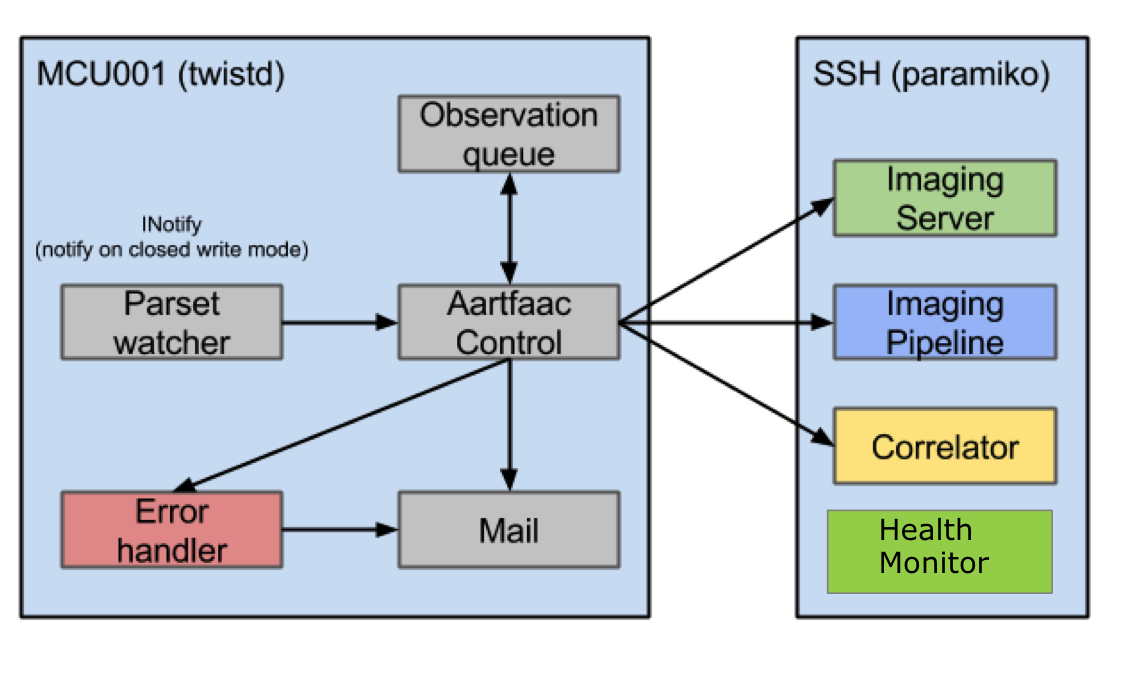
\includegraphics[width=0.5\textwidth]{Figs/control_sys.png}
\caption{The  control  system  architecture  which  interfaces  with  the  LOFAR
  observation scheduling system and triggers AARTFAAC observations.}
\label{fig:afaac_ctrl_sys}
\end{figure*}
The  AARTFAAC  control subsystem  coordinates  the  diverse processing  and  I/O
infrastructure of  the AARTFAAC system, and  acts as a liason  between the LOFAR
observatory,  AARTFAAC user  and  system.   It is  essential  to the  autonomous
functioning of  the instrument by  providing fault  tolerance.  It has  a python
based client-server architecture, with the  server process existing on the LOFAR
manager node and clients waiting for  commands on the various AARTFAAC subsystem
controllers. Every scheduled  LOFAR observation is monitored  for suitability as
an AARTFAAC observation. When such an observation is found, commands are sent to
the target subsystems  over TCP connections to dedicated  ports.  The sequential
execution   allows   parsing   of   process  outputs,   and   reinitiation,   if
necessary. Successful  execution of an  AARTFAAC observation is reported  to the
administrators via email.  Figure  \ref{fig:afaac_ctrl_sys} shows the functional
blocks  of  the AARTFAAC  control  system,  and  their  interface to  the  LOFAR
scheduling system.\\  

\noindent \textbf {Monitoring interface:} The control system allows monitoring the various
subsystems at fine granularity, making it useful to localize problems within the
system. A Munin[ref]  based system monitoring tool allows  viewing statistics of
I/O  between  nodes,   computing  on  various  nodes,  and  disk   usage  via  a
webpage(\footnote{https://proxy.lofar.eu/aartfaac/index.html}), including  history at  various time
cadences.  The processed  outputs at  various stages  in the  pipeline are  also
presented onto a webpage for the end  to end, and astronomical monitoring of the
system, some examples of this are shown in the results section.

\section {\label{sec:results} Commissioning results}
\begin{figure*}[htbp]
 %% \subfloat
   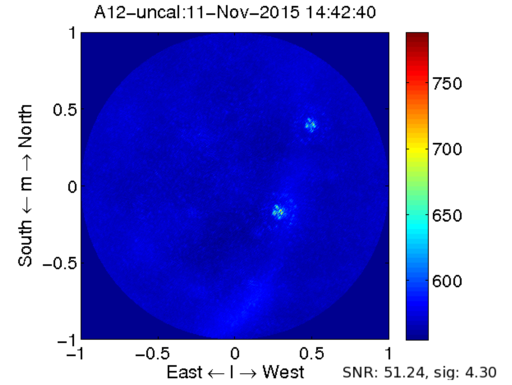
\includegraphics[width=0.5\textwidth]{Figs/A12_uncal.png}
 %% \subfloat 
 %%  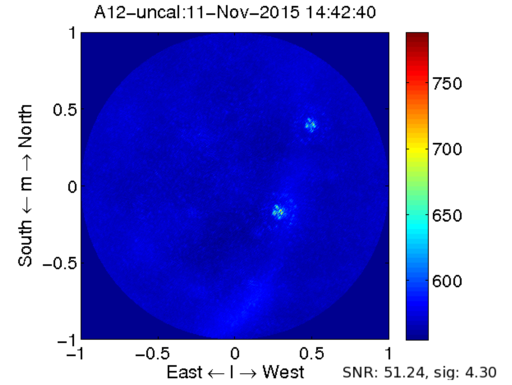
\includegraphics[width=0.3\textwidth]{Figs/A12_uncal.png}
\caption{An uncalibrated image from the 12-station AARTFAAC system, demonstrating the hardware data routing and  correlator functioning.}
\label{fig:afaac_results}
\end{figure*}
The AARTFAAC system is currently in place and operating with 6 LOFAR stations, a
total bandwidth of  ~3MHz, with real-time images being created  at a 1sec/192kHz
cadence. The correlator has been tested  to operate at the full specification of
12  stations  and  ~6MHz  bandwidth.  Fig.   \ref{fig:afaac_results}  shows  the
resulting All-sky snapshot image from the AARTFAAC monitoring webpage interface.

% \begin {itemize}
% \item {Overall latency of the system}
% \item {Long term performance of the entire system based on logs.}
% \item {Performance  in various  bit-modes, with  different number  of subbands,
%   expected sensitivity.}
% \item {Imaging quality Vs. latency: 6 station to 12 station.}
%\end {itemize}

\section {\label{sec:discussion} Discussion}
\begin{wstable}[h]
\caption{Overall latency budget and performance of AARTFAAC subsystems.}
\begin{tabular}{@{}cccc@{}} \toprule
Parameter & Compute time (ms) & Processing (TFLOPs)\\ \colrule
CPU data transform & 16.7 &0.1626  \\
GPU FFT & \hphantom{0}10.0&0.678  \\
GPU Delay and Bandpass correction & 2441.0 & 0.0\tnote{a}  \\
GPU correlation & 212.9 & 4.824\tnote{a}  \\ \colrule
\end{tabular}
\begin{tablenotes}
\item[a] Sample table notes.
\item[b] Sample table notes.
\end{tablenotes}
\label{tab:afaac_specs}
\end{wstable}

\noindent \textbf {Signal Processing requirements:}
A variety  of signal processing  algorithms are  utilized in the  generation and
analysis of  real-time images from  AARTFAAC.  Here,  we describe only  the ones
relevant to  the real-time performance  of the  system, i.e., not  including the
characterization   of  transients,   and   only   discuss  their   computational
requirements.  Their  implementation and  performance  can  vary based  on  data
dimensions and its match to a particular computing architecture.

The first signal processing block is the Polyphase Filterbank, which essentially
consists of  an FIR  filter followed by  an FFT. This  filter splits  the signal
spectrally with a  lower scalloping and spectral aliasing loss.  The filter bank
can  be  represented by  TODO  Muls  and TODO  accs,  leading  to a  theoretical
requirement of TODO FLOPs for N. The FFT has a compute load of TODO FLOPs.

The subbanded signal is usually further filtered to a higher spectral resolution
by  a second  stage  filterbank. The  delay and  bandpass  correction involve  a
complex multiplication of  the signal with a static weight  vector, leading to a
load  of  TODO FLOPs  per  subband  for  TODO  output spectral  resolution.  The
correlation  is  carried  out  at   the  output  spectral  resolution.  For  our
specifications, this leads to a load of TODO FLOPs per channel per timeslice.

The Calibration  is the only data  dependent, iterative operation to  be carried
out in the  real-time chain. It consists of mainly  TODO matrix operations, each
costing  TODO.  The  total  expected  cost of  calibration  is  TODO  FLOPs  per
covariance matrix, assuming an average of TODO major and TODO minor cycles.

The Imaging consists of a weighting  operation on all visibilities, per spectral
unit. This  corresponds to a  cost of  TODO FLOPs/channel/sec. The  weighting is
followed by a gridding of the calibrated  visibilities onto a grid whose size is
dependent on  the image resolution  and field of view,  and with a  kernel whose
size is  also dependent on output  resolution. For our TODO  typical parameters,
this translates to  a cost of TODO  FLOPs. The generated images need  to be flux
calibrated, which  corresponds to  an element by  element multiplication  with a
correction matrix. This cost is about TODO FLOPs.

Once  the calibrated  images are  available, they  are passed  through a  source
finding stage, where islands of emission  are isolated into (point) sources, and
their properties ascertained by fitting 2D Gaussians to the emission island. The
source parameters are then recorded into a database for every timeslice, and the
timeseries is further analysed for variability and for detecting transients.

\noindent \textbf  {Parallization axis:}  Parallelization to handle  the compute
requirements can be carried out along  the temporal, spectral or spatial axis of
the incoming  data.  Organizing timeslices  for parallel processing can  lead to
latencies, which is inconsistent with the real-time requirement of AARTFAAC. The
spatially  distributed dipoles  result  in each  dipole  stream being  initially
processed  independently of  each other.   The correlation  process retains  the
spatial independence  since the generated  covariance matrix can be  split along
dipoles.   However,  the  processing  requires  alignment  along  the  time  and
frequency axis,  and further analysis  (imaging) fuses the spatial  axis.  Thus,
the  frequency axis  is  the  only truly  independent  axis  along the  complete
processing chain, with each subband or channel being processed independently.

Parallelization at different levels in the hierarchy is matched to the available
hardware architecture.  At upstream levels, the FPGAs operate in lock-step, with
no dynamic scheduling of data to processing units. An important task here is the
reorganizing of data along the frequency  axis such that the architecture of the
computationally intense components (correlation) can be fully utilized.

Since the data from all dipoles is time and frequency aligned when correlation occurs,
   parallelization  is
fundamentally  on  the  frequency  axis,   with  each  subband  being  processed
independently.  Within a  subband, each station data  is processed independently
till the correlation  stage, where a synchronization barrier is  applied to time
align all the dipole streams.  Each channel of the subband correlation matrix is
also processed independently via a GPU  thread group.  Further, a single channel
covariance matrix is broken into cells, which are also computed independently.\\


\noindent \textbf {System performance:} The overall performance of the real-time
system is quantified by the achieved latency, and any drops in throughput due to
intermittent processing delays. Our overall average latency has been found to be
TODO secs, while throughput is maintained due to bounded processing. The breakup
of   the   latency,   and   associated   computing   is   presented   in   Table
\ref{tab:overall_perf}.\\

\noindent  \textbf   {AARTFAAC  Scalability:}   The  AARTFAAC   All-Sky  monitor
implementation  can be  scaled  up  along the  spatial  (number  of dipoles)  or
spectral (processed subbands) dimensions. A  spectral scaling will ultimately be
limited by the ring network bandwidth to  about 64 subbands (~12 MHz) of 8-bits,
doubling the current  bandwidth. A spare 10Gbps link on  the uniboards can bring
the extra  32 subbands to the  center, where they  can be processed by  an exact
duplicate of  the current correlator system.  The choice of a  hierarchical data
transpose results  in the most efficient  final layout for correlation.   In the
generic  case,  following   the  same  design,  additional   subbands  could  be
accomodated by increasing the levels in  the network hierarchy to accomodate the
transpose.   The final  correlation would  then be  possible for  the additional
subbands by replication of the frequency multiplexed hybrid correlator.

Keeping the  current bandwidth while increasing  the number of input  dipoles is
also  feasible. The  infiniband  interface  allows another  two  stations to  be
added.  The compute  requirements  would be  almost 30\%  higher,  due to  their
quadratic growth  with number of  input streams.  The correlation  operation has
been tested on the current GPUs for scalability of the input streams, and should
be  able to  cope  with  the requirements  of  the  extra inputs.  Accommodating
stations in addition to  the two mentioned here would likely  require data to be
transferred  between  multiple  CPUs  over  the  GigE  network,  which  will  be
prohibitively slow.\\

\noindent  \textbf {Impact  of sharing  dipoles with  LOFAR on  AARTFAAC:} LOFAR
operates using  either the LBA  or the  HBA antenna at  a time. Further,  due to
limited station level electronics for stations within the core, only a subset of
the available  station dipoles can be  utilized. This implies that  the AARTFAAC
telescope  is  dependent  on  LOFAR  for  the  choice  of  antenna  and  station
configuration,  reducing the  availability  for all-sky  monitoring. Within  the
station, only the LBA\_OUTER station configuration is currently deemded suitable
for  real-time imaging.   This mode  of  LOFAR operation  favorable to  AARTFAAC
depends on  the observing  schedule and the  proposed observations.   Table TODO
shows some  statistics from previous cycles  on the fraction of  observing modes
favorable to AARTFAAC. Based on this, it  may be resonable to expect AARTFAAC to
operate TODO fraction of time, typically.\\

\noindent \textbf {Hierarchical  shuffling and transpose of  incoming data:} The
voltages  are available  as a  sampled  timeseries per  polarization, with  time
samples laid out contiguously in memory.  For efficient computing, these need to
be transposed such that the same  timeslice from all dipoles lie contiguously in
memory. This  operation involves transposing a  matrix of data with  a size NxN,
with N  being the  number of data  sources.  This memory  becomes inflated  by a
factor corresponding  to the number of  timesamples in the integration  unit, as
well as the number of polarizations  being processed. Since the memory footprint
can be quite  large, this is quite  an inefficient operation due  to memory read
latencies etc.\\

We achieve this by spreading the transpose operation over the nodes
on our network. This is done in the following manner:
The URI boards carry out a first  level of transposition by physically routing a
subbands  from a  group  of 4  dipoles  to  a single  output.  The second  stage
transpose is  carried out  by the Uniboard.  This is at  the station  level, and
routes  all dipole  data from  one  station as  a contiguously  laid out  group.
Finally, the inter-station transpose to reorder  data and exchange the time axis
for  the  station  axis  is  carried  out by  the  CPU  host  component  of  the
correlator. Here, the  PC memory is used  to rearrange the incoming  data and to
carry out  the transform. The  resulting output is  then optimally laid  out for
correlation over all  dipoles of the AARTFAAC, for every  polarization, and over
the chosen integration time range.

%\subsection {Dynamic range and precision of computing}
%The 12-bit sampling (TODO: Confirm) provides  for a dynamic range of TODO. These
%raw data samples  are fed into the  hardware first stage PFB,  which carries out
%internal computation  on TODO bit  integer data,  and generates 16-bit  or 8-bit
%complex components (TODO: Is there any normalization at this stage? Why else are
%the actual numbers  so high?). Due to each dipole  sampled output being directly
%operated on without  any beamforming, the 8-bit dynamic range  has been found to
%be adequate for the AARTFAAC application.  Once the data reaches the correlator,
%all computations are carried out with single precision floating points.

\section {\label{sec:conclusion} Conclusions}
We  describe the  AARTFAAC All-sky  radio transient  monitor, an  autonomous and
real-time image  domain transient detection  machine piggy-backing on  the LOFAR
radio telescope. The  system consists of a diversity  of heterogenous subsystems
ranging  from  FPGA  firmware,  to   heterogenous  GPGPU  machines,  with  final
processing carried out on commodity computing  machines.  Its aim is to generate
real-time  triggers on  the detection  of reliable  transients, to  enable their
multi-wavelength followup.

Our implementation utilizes  a hierarchical routing of high bandwidth  data to a
central  correlator,  with co-processing  within  the  hierarchy to  spread  the
computing cost.  The most intesive computing  of the correlations of  1152 input
streams requires $\sim$ 17TFLOPs, and has  been achieved on a system consisting of
10  state-of-the-art GPUs.  Our system  operates in  real-time, with  an average
latency of TODO  seconds to the imaging, while generating  images with a dynamic
range of close to 2000:1 with a time and spectral integration of 1sec/190kHz.

The scalability of  this system demonstrates the viability of  handling an SKA-1
like  sea-of-antennas approach  to enable  wide field  radio monitoring  at high
sensitivity.\\

\noindent \textbf{Acknowledgements}
This work is funded by the ERC grant C.2320.0056 awarded to Prof.  Ralph Wijers,
University  of Amsterdam. We  thank The  Netherlands  Foundation for  Radio
Astronomy  (ASTRON)  for support  provided  in  carrying out  the  commissioning
observations.

\bibliographystyle{ws-jai}
\bibliography{ref}

\end{document} 
